\section{Zielsetzung}
\label{sec:Zielsetzung}

In diesem Versuch soll die Herauslösung von Elektronen aus Metallen (hier: Wolfram)
mithilfe des glühelektrischen Effekts untersucht werden. Von besonderem Interesse
ist hier die Temperaturabhängigkeit dieses Effekts.

\section{Theorie}
\label{sec:Theorie}

\subsection{Leitungselektronen in Metallen}

Metalle haben eine Gitterstruktur und eine sehr gute 
elektrische Leitfähigkeit, welche durch die auf dem 
Kristallgitter sitzenden ionisierten Atome zu begründen
ist.
Die Ionen sind durch diese Gitterstruktur räumlich
periodisch verteilt und werden von freigesetzte Elektronen
eingehüllt, welche keinem bestimmten Atom mehr zuzuordnen
sind. Sie befinden sich stattdessen im Kraftfeld sämtlicher
Atome in dem Kristallgitter.
Diese Elektronen werden \textit{Leitungselektronen} genannt.
Die Ionen stellen durch die Abwesenheit der Elektronen
eine positive Ladungsquelle dar. Daher nimmt das Gitterpotential
in der Nähe dieser Gitterpunkte hohe positive Werte an.
Weiter entfernt ist das Potential allerdings näherungsweise
konstant.

Mit dieser Näherung kann das Metallinnere als ein Gebiet
angesehen werden, in dem ein konstantes positives Potential
herrscht. Dieses Potential ist um den Betrag $\xi$
vom Außenraum verschieden. Damit Elektronen das Metall
verlassen können, müssen diese also eine Potentialbarriere
der Höhe $\xi$ überwinden. Dargestellt ist dies 
in \autoref{Abb:Potentialtopf}.\\

\begin{figure}[H]
    \centering
    
    \caption{Potentialtopf-Modell eines Metalls.\cite{sample}}
    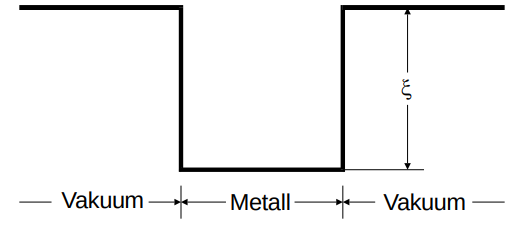
\includegraphics[width=\textwidth]{Bilder/Potentialtopf.png}
    \label{Abb:Potentialtopf}
\end{figure}

\subsection{Austrittsarbeit der Elektronen}

Um gegen dieses Potential anlaufen zu können, muss eine
\textit{Austrittsarbeit} $\mathrm{e}_0 \xi$ geleistet
werden. Die Konstante $\mathrm{e}_0$ ist hier die
Elementarladung.
Es stellt sich nun die Frage, ob die Elektronen dieses
Potential ohne zusätzliche Energie Zufuhr verlassen können.
Also ob die innere Energie der Elektronen hoch genug ist.
Die Quantentheorie liefert hier eine zufriedenstellende 
Antwort:\\
Aus der Quantentheorie wissen wir, dass Elektronen 
nur bestimmte Energiewerte $E_{\mathrm{n}}$ annehmen können.
